\documentclass{article}

\usepackage{graphicx}
\usepackage{tikz}
\usepackage{tikzsymbols}
\usetikzlibrary{calc,patterns,shapes.geometric}
\pagestyle{empty}
\usepackage[margin=0pt]{geometry}
\geometry{papersize={14in,12in}}

\def\centerarc[#1](#2)(#3:#4:#5){\draw[#1] ($(#2)+({#5*cos(#3)},{#5*sin(#3)})$) arc (#3:#4:#5);}

\begin{document}
	\begin{figure}
		\centering
		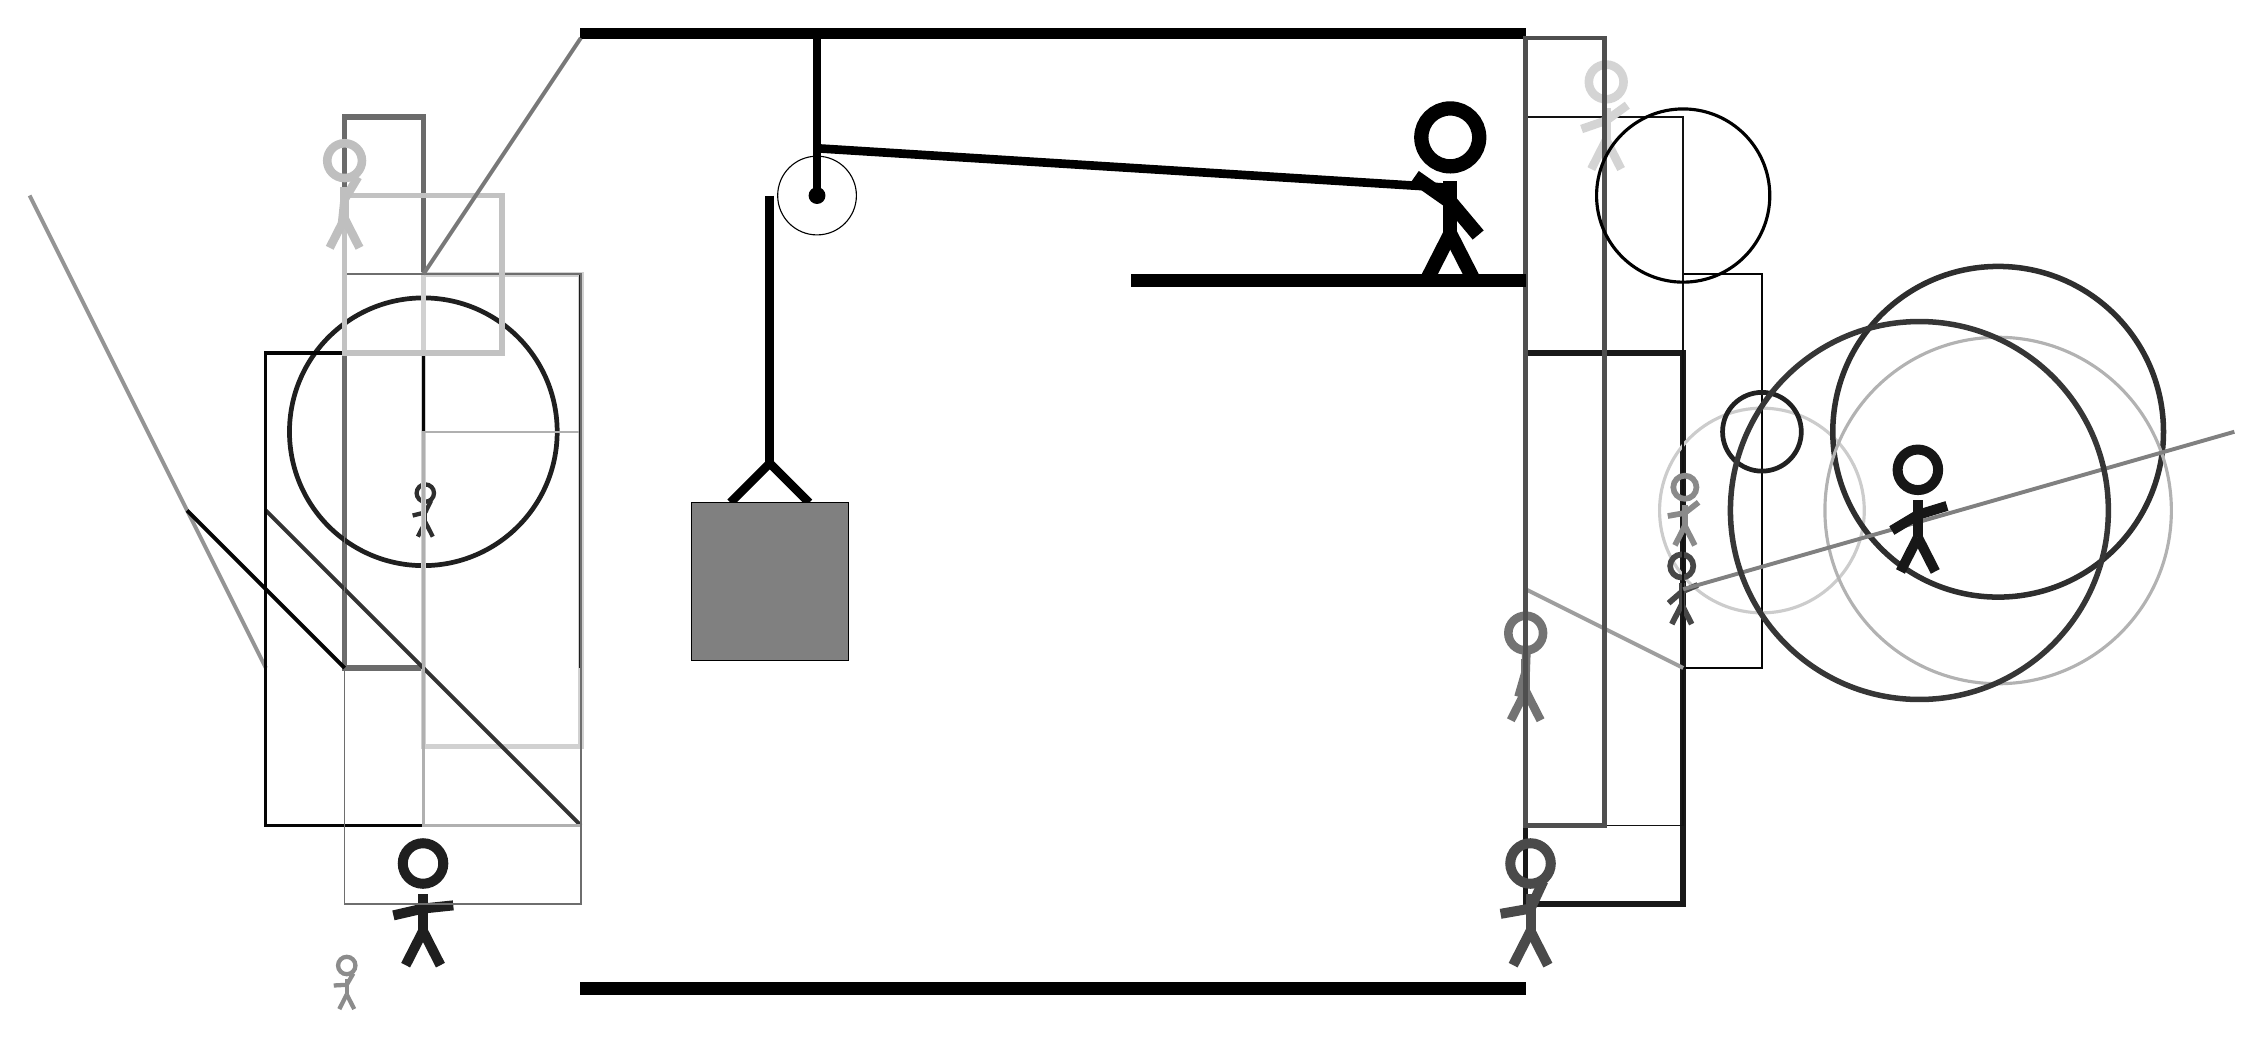
\begin{tikzpicture}
			%%%%% START %%%%%
			
			\draw[fill=black] (-2, 9) rectangle (10, 9.125);
			
			\draw[line width=0.7mm, color=black!90] (10, 5) rectangle (12, -2);
			
			\draw[line width=0.3mm, color=black!98] (12, 1) rectangle (13, 6);
			\node[line width=0.3mm, color=black!71] at (10, -2) {\Strichmaxerl[7][10][65]};
			\draw[line width=0.5mm, color=black!42](-6, 1) -- (-9, 7);
			\draw[line width=0.7mm, color=black!58] (-4, 1) rectangle (-5, 8);
			\draw [line width=0.4mm, color=black!20](13, 3) circle (1.3);
			\node[line width=0.5mm, color=black!82] at (-4, 3) {\Strichmaxerl[3][14][64]};
			\draw [line width=0.7mm, color=black!82](16, 4) circle (2.1);
			\node[line width=0.6mm, color=black!72] at (12, 2) {\Strichmaxerl[4][41][23]};
			
			\node[line width=0.6mm, color=black!45] at (-5, -3) {\Strichmaxerl[3][3][60]};
			
			\draw [line width=0.4mm, color=black!30](16, 3) circle (2.2);
			\draw [line width=0.6mm, color=black!88](-4, 4) circle (1.7);
			\draw[line width=0.7mm, color=black!18] (-4, 0) rectangle (-2, 6);
			
			\draw[line width=0.2mm, color=black!93] (12, 8) rectangle (10, -1);
			\draw[line width=0.5mm, color=black!50](12, 2) -- (19, 4);
			\draw [line width=0.6mm, color=black!87](13, 4) circle (0.5);
			\node[line width=0.6mm, color=black!91] at (15, 3) {\Strichmaxerl[7][31][17]};
			\draw[line width=0.5mm, color=black!80](-6, 3) -- (-2, -1);
			\draw[line width=0.4mm, color=black!98] (-4, 5) rectangle (-6, -1);
			\node[line width=0.5mm, color=black!88] at (-4, -2) {\Strichmaxerl[7][13][6]};
			\draw[line width=0.3mm, color=black!31] (-4, -1) rectangle (-2, 4);
			
			\draw [line width=0.7mm, color=black!79](15, 3) circle (2.4);
			\draw[line width=0.4mm, color=black!88] (-2, 6) rectangle (-2, 1);
			\draw[line width=0.2mm, color=black!57] (-2, 6) rectangle (-5, -2);
			\draw[line width=0.7mm, color=black!24] (-3, 5) rectangle (-5, 7);
			\node[line width=0.7mm, color=black!46] at (12, 3) {\Strichmaxerl[4][10][38]};
			\node[line width=0.4mm, color=black!25] at (-5, 7) {\Strichmaxerl[6][84][59]};
			\draw[line width=0.5mm, color=black!53](-2, 9) -- (-4, 6);
			
			\node[line width=0.2mm, color=black!55] at (10, 1) {\Strichmaxerl[6][74][88]};
			\draw[line width=0.5mm, color=black!38](10, 2) -- (12, 1);
			\node[line width=0.2mm, color=black!17] at (11, 8) {\Strichmaxerl[6][19][36]};
			
			\draw[line width=0.6mm, color=black!69] (11, -1) rectangle (10, 9);
			\draw [line width=0.4mm, color=black!100](12, 7) circle (1.1);
			\draw[line width=0.5mm, color=black!98](-7, 3) -- (-5, 1);
			
			
			\draw (1, 7) circle (0.5);
			\draw[fill=black] (1, 7) circle (0.1);
			\draw[line width=1.1mm] (1, 9) -- (1, 7);
			
			\draw[line width=1.1mm](-0.1, 3.1) --  (0.4, 3.6) -- (0.9, 3.1);
			\draw[fill=black!50] (-0.6, 3.1) rectangle (1.4, 1.1);
			
			\draw[line width=1.1mm](0.4, 7) -- (0.4, 3.6);
			\centerarc[line width=1.1mm](1, 7)(90:180:0.6)
			\draw[line width=1.1mm](1, 7.6) -- (9, 7.1);
			
			\node at (9, 7) {\Strichmaxerl[10][-35][-50]};
			\draw[fill=black] (5, 6) rectangle (10, 5.85);
			
			\draw[fill=black] (-2, -3) rectangle (10, -3.15);
			
			%%%%% END %%%%%
		\end{tikzpicture}
	\end{figure}	
\end{document}